
\begin{figure}[h]
\centering
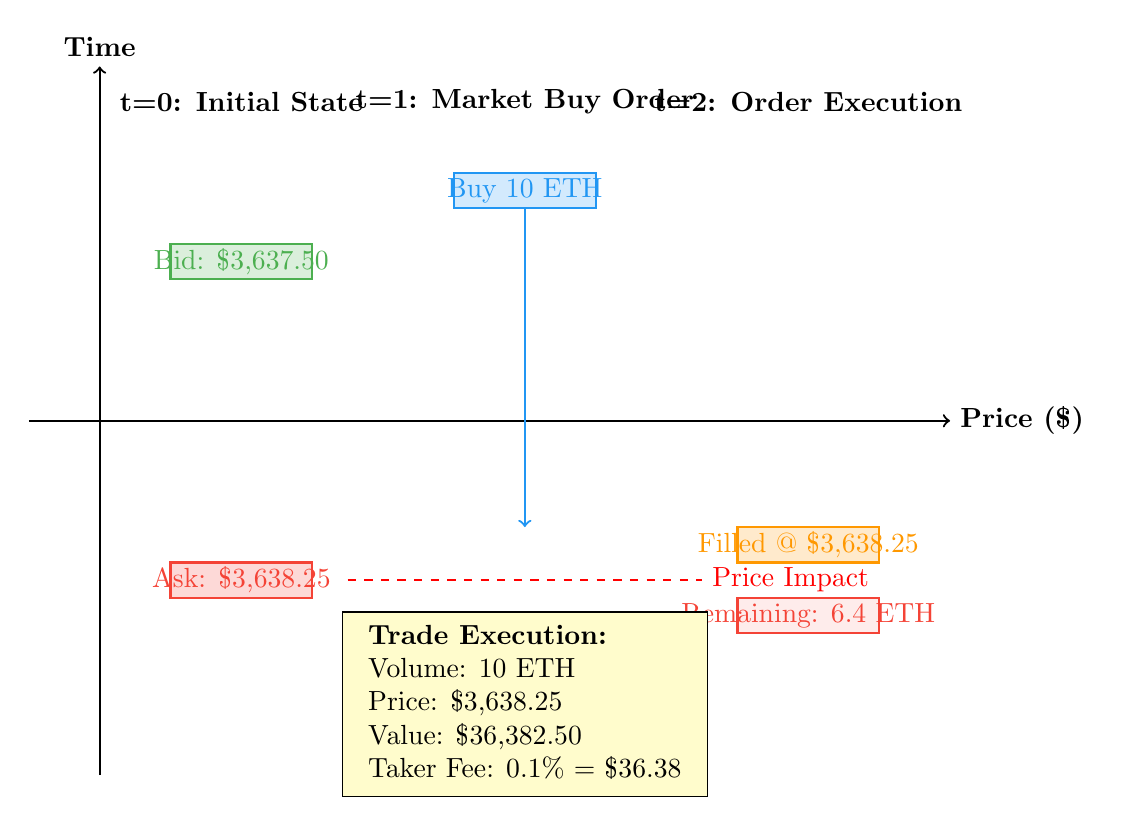
\begin{tikzpicture}[scale=0.9]
% Define colors
\definecolor{bidcolor}{RGB}{76, 175, 80}
\definecolor{askcolor}{RGB}{244, 67, 54}
\definecolor{neworder}{RGB}{33, 150, 243}
\definecolor{execution}{RGB}{255, 152, 0}

% Timeline
\draw[->, thick] (0, -5) -- (0, 5) node[above] {\textbf{Time}};
\draw[->, thick] (-1, 0) -- (12, 0) node[right] {\textbf{Price (\$)}};

% Initial order book state (t=0)
\node at (2, 4.5) {\textbf{t=0: Initial State}};
\draw[bidcolor, thick, fill=bidcolor!20] (1, 2) rectangle (3, 2.5) node[midway] {Bid: \$3,637.50};
\draw[askcolor, thick, fill=askcolor!20] (1, -2) rectangle (3, -2.5) node[midway] {Ask: \$3,638.25};

% Market buy order arrives (t=1)
\node at (6, 4.5) {\textbf{t=1: Market Buy Order}};
\draw[neworder, thick, fill=neworder!20] (5, 3) rectangle (7, 3.5) node[midway] {Buy 10 ETH};
\draw[->, neworder, thick] (6, 3) -- (6, -1.5);

% Execution (t=2)
\node at (10, 4.5) {\textbf{t=2: Order Execution}};
\draw[execution, thick, fill=execution!20] (9, -1.5) rectangle (11, -2) node[midway] {Filled @ \$3,638.25};
\draw[askcolor, thick, fill=askcolor!10] (9, -2.5) rectangle (11, -3) node[midway] {Remaining: 6.4 ETH};

% Trade details
\node[rectangle, draw, fill=yellow!20] at (6, -4) {
\begin{tabular}{l}
\textbf{Trade Execution:} \\
Volume: 10 ETH \\
Price: \$3,638.25 \\
Value: \$36,382.50 \\
Taker Fee: 0.1\% = \$36.38
\end{tabular}
};

% Market impact illustration
\draw[red, thick, dashed] (3.5, -2.25) -- (8.5, -2.25) node[right] {Price Impact};

\end{tikzpicture}
\caption{Market Order Matching Process. A market buy order for 10 ETH executes against the best ask at \$3,638.25, demonstrating immediate liquidity consumption and price impact in the ETH/USDC order book.}
\label{fig:market_order_matching}
\end{figure}
